\documentclass{amsart}
\usepackage{hyperref}
\usepackage{graphicx}

%% Aliases
\DeclareMathOperator{\notmodels}{\nvDash}  %% Requires amssymb package

\DeclareMathOperator{\Feventually}{\rotatebox[origin=c]{45}{$\Box$}}
\DeclareMathOperator{\Galways}{\Box}
\DeclareMathOperator{\Xnext}{\bigcirc}
\DeclareMathOperator{\Uuntil}{\mathbf{U}}


%% Denote the set of all states satisfying the formula.
%% Courtesy of Pavithra Prabhakar; Aug 2012.
\newcommand{\sem}[1]{\ensuremath{[\![#1]\!]}}


\theoremstyle{definition}
\newtheorem{example}{Example}[section]


%% format is YYYY-MM-DD
\def\now{\number\year%
-{\ifnum \month < 10 0\fi}\number\month%
-{\ifnum \day < 10 0\fi}\number\day}

\begin{document}
\title{A competition on formal methods for robotics}
\author{Scott C. Livingston}
\author{Vasumathi Raman}
\date{\textbf{DRAFT} \now}
\begin{abstract}
This is the normative reference for the first challenge on formal methods for
robotics.  Formal methods refers broadly to techniques for the verification and
automatic synthesis of transition systems that satisfy desirable properties
exactly or within some statistical tolerance.  Though historically developed for
concurrent software, recent work has brought these methods to bear on motion
planning in robotics.  Challenges specific to robotics, such as uncertainty and
real-time constraints, have motivated extensions to existing methods and
entirely novel treatments.  However, compared to other areas within robotics
research, demonstrations of formal methods have been surprisingly small-scale.
The proposed robotics challenge seeks to motivate advancement of the state of
the art toward practical realization.  The challenge is organized into three
problem domains: arbitrary dimensional chains of integrators, roads with Dubins
cars, and manipulation tasks on the assembly line.
\end{abstract}
\maketitle


\section{Introduction}

We present the first challenge on formal methods for robotics, which will
henceforth be referred to simply as ``the Challenge.''  It is to be hosted at
the International Conference on Robotics and Automation ({ICRA}) in May 2015.
The purpose of this document is to describe in detail the Challenge, including
the problem domains, rules, and scoring procedures.  Unless explicitly stated
otherwise, the description herein is normative.

\section{Summary (not normative)}

The challenge will consist of three problem domains that touch on a diversity of
difficulties one would need to address in a practical deployment.  These problem
domains together involve many fronts of current work in formal methods for
robotics.  To avoid requiring too general of a solution---and in particular, to
improve accessibility for a broad group of potential competitors---entries to
the challenge are permitted to select a subset of these domains.  More
precisely, each team may enter any number of control programs, each of which may
be used on any subset of the problem domains.  Results of the challange will be
organized by problem domains.  Control programs that are used in multiple
domains will receive total scores as the sum of scores from each attempted
domain.  The intent in the scoring structure will be to have excellent
performance in a single problem domain regarded as being comparable to good
performance in all domains.  Teams will be able to trade-off generality with
problem-specific tuning.

In the preparation materials to be made available for potential competitors, we
will release elementary solutions to complete each domain.  These will establish
feasibility of the problems, provide reference implementations for the challenge
execution framework, and give teams something on which to build, should they
choose to do so.


\section{Preliminaries (not normative)}

This section introduces notation used throughout the paper.  It also gives brief
introduction to concepts that may not be widely known by potential participants
at ICRA.  Let $A$ be a set.  $2^A$ denotes the set of all subsets of $A$.  The
set of nonnegative real numbers is denoted by $\mathbb{R}_{\geq 0}$.  Let
$x=(x_1 , \ldots, x_n )\in \mathbb{R}^n$.  For $p \geq 1$, the $p$-norm of $x$
is defined to be
\begin{equation}
\lVert x \rVert_{p} = \left( \sum_{i=1}^{n}\lvert x_i \rvert^{p} \right)^{1/p} .
\end{equation}
The $2$-norm is also known as the Euclidean distance.  The $\infty$-norm is
defined as
\begin{equation}
\lVert x \rVert_{\infty} = \max_{i}\lvert x_i \rvert .
\end{equation}

Linear-time temporal logic (LTL) is an extension of Boolean (or propositional) logic
that describes properties for countably infinite sequences of events.  The two
basic temporal operators are $\Uuntil$ (pronounced ``until'') and $\Xnext$
(pronounced ``next''). $\psi \Uuntil \varphi$ requires that the formula $\psi$
holds until a state satisfying $\varphi$ is reached and such a state must
eventually be reached.  The operator $\Galways$ is also used; informally,
$\Galways \psi$ requires $\psi$ is satisfied by all states reached during an
execution.  Intuitively the operator $\Feventually$ is dual to $\Galways$;
informally, $\Feventually \psi$ requires that a state satisfying $\psi$ occurs
in finite time.

A convex polytope is a bounded region defined by the intersection of finitely
many halfspaces, each of which is defined by a linear inequality.  There are
many useful computations known for polytopes, many of which are fast, e.g.,
intersection. \cite{Fukuda2004}

The discrete notions of temporal logic are related to the real-valued spaces of
continuous dynamical systems as follows.  Suppose a state space contains
finitely many polytopes, and each polytope is regarded as labeled.  A trajectory
through this space is labeled with the sequence of polytopes with which it
intersects.


\section{Terminology}

A \textit{team} is the basic entity that can compete and, depending on
performance, receive rankings in the Challenge.  A team must have a name by
which it will be referred to during the Challenge.

There are three \textit{problem domains}, which are described in
Sections~\ref{sec:scalingcinteg}, \ref{sec:trafficdubins}, and
\ref{sec:dexterousmanip} (one per section).  Within a problem domain, a problem
\textit{instance} is a particular workspace, arrangement of obstacles, labeling
of the workspace, selection of parameters for the robot dynamics, and a task
formula.

Each problem domain may have one or more \textit{variants}, which concern
different manners of implementation or random instance generation.  E.g., the
traffic of Dubins cars domain (cf.\ Section~\ref{sec:trafficdubins}) has a
simulation variant, which relies on Gazebo, and a physical variant, which
involves a real testbed of several Kobuki bases as well as an overhead pose
tracking system.

A \textit{controller} is the basic entity that a team submits for the Challenge
within a particular problem domain.  Each controller is scored and ranked, and
the score of a team is simply the maximum score of any controller belonging to
that team.


\section{Procedure}

The scaling chains of integrators (Section~\ref{sec:scalingcinteg}) domain
will proceed entirely in simulation.  The other two domains (described in
Sections~\ref{sec:trafficdubins} and \ref{sec:dexterousmanip}) will include both
simulation and physical variants.


\section{Problem domain: Scaling chains of integrators}\label{sec:scalingcinteg}

The first problem domain is the simplest in terms of dynamics and
specifications, yet unlike the other domains, the system to be controlled can be
scaled easily to arbitrarily many dimensions.  While this problem is abstract in
the sense that it is not modeling a specific physical system, it is
well-motivated because the double-integrator is just the basic force equation of
Newtonian mechanics, up to a scaling factor.  Informally, this problem domain
concerns controlling acceleration or a higher order derivative of a point-mass
in high-dimensional spaces so as to visit goal regions and avoid obstacles.  The
precise description is given below.

\subsection{Dynamics and constraints}

Let $n$ and $m$ be positive integers.  Consider the differential equation
\begin{equation}\label{eq:minteg}
D^{m}q = u ,
\end{equation}
where $q: [0,\infty [ \rightarrow \mathbb{R}^{n}$ and $D$ is the differential
operator.  The input $u$ is bounded as $\lVert u(t) \rVert_1 \leq
u_{\mathrm{max}}$.  The system is called a \textit{chain of a integrators}
because it can be rewritten as a linear control system
\begin{equation}\label{eq:cintegdyn}
\begin{split}
\dot{x}_1 &= x_2 \\
\dot{x}_2 &= x_3 \\
&\vdots \\
\dot{x}_{m-1} &= x_m \\
\dot{x}_m &= u \\
y &= x_1
\end{split}
\end{equation}
where for time $t$, each $x_{i}(t)\in \mathbb{R}^n$ for $i=1,\ldots,m$, and
$x(t)=\left( x_{1}(t) , \ldots , x_{m}(t)\right)\in \mathbb{R}^{nm}$. The output
trajectories of \eqref{eq:cintegdyn} are exactly those of \eqref{eq:minteg},
given the same input, and thus we call them equivalent. In \eqref{eq:minteg},
control input is applied as the $m$-th derivative of an $n$-dimensional variable
$q$, and the intermediate derivatives are made explicit in
\eqref{eq:cintegdyn}. A notable particular case is $m=2$, which is called the
``double integrator''. If $n \leq 3$ then $q$ may be referred to as the
``position''.

To introduce process and sensor noise, consider the 2-dimensional system
\begin{align}
\dot{x} &= \left(
\begin{array}{cc}
0 & 1 \\
0 & 0
\end{array}
\right) x + \left(
\begin{array}{c}
0 \\
1
\end{array}
\right) u + \xi \label{eq:dintegdyn}\\
y &= \left(
\begin{array}{cc}
1 & 0
\end{array}
\right) x + \eta \label{eq:dintegobs},
\end{align}
where $\xi$ and $\eta$ are either bounded disturbances (nondeterministic) or
stochastic processes.  Equivalence with \eqref{eq:minteg} in the case of
$n=1, m=2$ and $\xi=\eta=0$ is apparent using $x_1 = q$ and $x_2 = \dot{q}$.  For $n
> 1$, the matrices in \eqref{eq:dintegdyn} and \eqref{eq:dintegobs} can be
repeated in block diagonal form to yield a new linear time-invariant system of
dimension $2n$ and which is again equivalent to \eqref{eq:minteg} for $m=2$.

\subsection{Specifications}

Task specifications will require visitation of regions while avoiding obstacles.
Compared with the specifications for the other problem domains presented in
Sections~\ref{sec:trafficdubins} and \ref{sec:dexterousmanip}, these can be
regarded as a slight extension beyond classical motion planning.  There are two
forms of specifications:
\begin{equation}\label{eq:dinteg-surveillance}
q(0) = \mathrm{init} \wedge \Galways \left( q(t) \notin \mathrm{Obs} \right) \wedge \bigwedge_{i} \Galways \Feventually \mathrm{goal}_i
\end{equation}
and
\begin{equation}\label{eq:dinteg-timedreach}
q(0) = \mathrm{init} \wedge \Galways \left( q(t) \notin \mathrm{Obs} \right) \wedge \bigwedge_{i} \left( \mathrm{counter}_i \leq T_{i} \right) \Uuntil \mathrm{goal}_i ,
\end{equation}
where $\mathrm{Obs} \subset \mathbb{R}^n$ is the obstacle set, which is
represented by a finite union of polytopes.  For each $i$, $\mathrm{counter}_i$
is a discrete clock that enforces the real-time deadline $T_i$ of reaching
region $\mathrm{goal}_i$.  Goal region $\mathrm{goal}_i$ is defined by a convex
polytope.  The initial position is a single point, $\mathrm{init}\in
\mathbb{R}^n$.  As part of the specification form \eqref{eq:dinteg-timedreach},
a time of initialization and rate of progression of the discrete counters is
specified.  These are significant because they determine in what order and how
quickly the goal regions must be reached.



\subsection{Implementation plan for the challenge}

This problem domain will be evaluated entirely within a numerical simulation.
As such, competitors will submit controllers for this part of the challenge
before the conference, and results will be obtained during live runs at ICRA.
After completion of each run in real-time, using software released as part of
the problem domain source code, animations will be generated to depict results.
In order to facilitate visualization of the results, each specification will consist 
of a conjunction of specifications, each of which governs no more than three 
dimensions of the state space. This enables plotting trajectories in these 3D 
subspaces, and visually verifying satisfaction of the specification. 

The main evaluation metric for this domain will be scalability of solutions to
high dimensions and large problem sizes. As such, we are currently investigating
feasibility of running the trials for this domain on common compute hardware,
such as through Amazon Web Services (\url{http://aws.amazon.com/}).


\section{Problem domain: Traffic network of Dubins cars}\label{sec:trafficdubins}

This domain involves navigation in a small network of two-lane roads with
vehicles that follow unicycle-like dynamics. Unlike the ``scaling
chains of integrators'' problem (cf.\ Section~\ref{sec:scalingcinteg}), now
there is an adversary that selects the motion of other cars.  The adversary is
subject to assumptions such as obeying traffic rules and not parking unfairly at
locations that must be eventually reached by the controller.

\subsection{Dynamics and constraints}
All cars including the controlled robot are assumed to have the same rigid body
shape and to have the same dynamics. Let $\mathcal I$ be the index set for the
cars in the network, with $r$ denoting the index of the controlled robot; all
cars indexed with $i \in {\mathcal I}\backslash\{r\}$ are regarded as a part of
the (adversarial) environment.

The pose of each car $i \in {\mathcal I}$ is specified by $(x_i,y_i,\theta_i)$,
where $(x_i,y_i)\in \mathbb{R}^2$ is referred to as \textit{position}, and
$\theta_i \in S^1$ is referred to as \textit{orientation}.  The car's body is a
rectangle or a circle, and the position is defined to be at the mean point
(center of mass) of the body.  Let $w$ be the width of the car -- this is
identical for each $i \in {\mathcal I}$.

The trajectories of car $i$ are solutions of
\begin{align}
\dot{x_i} &= u_i \cos \theta_i \\
\dot{y_i} &= u_i \sin \theta_i \\
\dot{\theta_i} &= \omega_i
\end{align}
where the control inputs are constrained as $u_i(t)\in \{0,u_{\mathrm{max}}\}$ and
$\omega_i(t) \leq \omega_{\mathrm{max}}$.


The workspace is a randomly generated road network constructed as follows.
Create a planar graph $G = (V,E)$ in which each vertex $v$ has degree $d_v \le 4$
(i.e., at most 4 neighbors).  Embed this graph in the plane, and expand the
edges to have width $4w$ (recall $w$ is the common vehicle width).

For this aspect of the ``traffic network of Dubins cars'' problem domain, we are
able to vary the bounds $u_{\mathrm{max}}$ and $\omega_{\mathrm{max}}$ on the
permissible control inputs, the size ($|V|$) and topology ($|E|$) of the road
network, and the number of other cars, i.e. $|\mathcal I|$.


\subsection{Specifications}

Because there is now an environment that may behave adversarially, task
specifications will be of the form $\varphi_{\mathrm{env}} \Rightarrow
\varphi_{\mathrm{sys}}$, where $\varphi_{\mathrm{env}}$ is known as the
``assumption'' and $\varphi_{\mathrm{sys}}$ as the ``guarantee.''  The desired
behaviors to be realized by the robot are provided through
$\varphi_{\mathrm{sys}}$ and include
\begin{enumerate}
\item obstacle avoidance while repeatedly visiting regions of interest, as in
  \eqref{eq:dinteg-surveillance};

\item reaching certain points within a time limit, e.g., as a model of deadlines
  for refueling, as in \eqref{eq:dinteg-timedreach};

\item remaining in the right-lane except when it is blocked;

\item stopping at intersections, which are treated as all-ways stops, and then
  proceeding based on order of arrival.
\end{enumerate}
The other cars will be assumed to follow the same road rules as listed above.
However, exceptions (violations) may occur, and thus additional fairness
assumptions will be provided, e.g.,
\begin{equation}\label{eq:freegoals}
\bigwedge_i \Galways \Feventually \tt{free}(\mathrm{goal}_i)
\end{equation}
which provides that other cars will always eventually vacate the $i$-th goal
region. The position of the other cars will be provided when in a predetermined 
radius, to simulate solving the associated vision problem. 

\begin{figure}[h!]\label{fig:network}
  \centering
        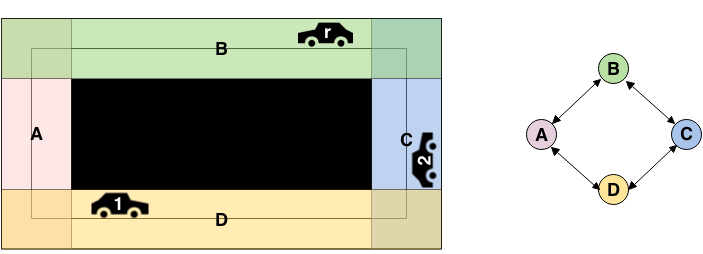
\includegraphics[width=1.0\textwidth]{images/network}
  \caption{An example road network and the graph from which it was generated. There are three cars, one of which is the robot (labeled with $r$)}.
\end{figure}

\begin{example}
Consider the network depicted in Fig. \ref{fig:network}. There are three cars,
one of which is the robot to be controlled. The road network graph is depicted,
and shows the bidirectional connectivity between the four road segments $A$,
$B$, $C$ and $D$. Note that each road has two lanes. At the intersection of each
pair of roads, there is an overlap region.
\end{example}

TODO: what does the LTL specification look like for this problem?

\subsection{Implementation plan for the challenge}

We are currently exploring feasibility of simulation using CloudSim
(\url{http://cloudsim.io}), which was developed for running Gazebo-based
simulations (\url{http://gazebosim.org}) as part of the ``virtual'' component of
the current DARPA challenge (\url{http://www.theroboticschallenge.org}).

Besides simulation, we plan to construct a reduced size form of this challenge
domain for running on-site at ICRA.  Both the robot to be controlled and the
adversarial vehicles will be based on Kobuki mobile bases
(\url{http://yujinrobot.com/eng/?portfolio=kobuki}).  Because all
problem-relevant motion will occur within a fixed plane, high-speed overhead
pose tracking is possible using a single camera mounted on the ceiling.  We hope
to install such a system on-site at ICRA to provide ground truth positions for
scoring purposes, even if the data is not available to competitors during the
challenge.

\section{Problem domain: Dexterous manipulation on the assembly line}\label{sec:dexterousmanip}

This problem domain concerns pick and place tasks, expressed using LTL
contracts, as described below. The key challenges explored in this problem
domain will include uncertainty in the shape and dynamics of the end-effector,
as well as objects that are being grasped, and collision-avoidance with moving
obstacles that come into the workspace, including humans.

\subsection{Dynamics and constraints}
For the tasks in this problem domain, the robot workspace is a three-dimensional
Euclidean space. The focus is on picking up and moving objects around, but will not 
involve difficult grasping problems, like deformable surfaces. To this end, the end-effector
will be something easy to use, like a magnet or some suction mechanism, such as a 
Universal Jamming Gripper \cite{AmendBRJL12}.

TODO: dynamics of the arm


\subsection{Specifications}
The specified scenario will be as follows. The robot is to process objects laid out on a cart that 
is brought to it and sort them into bins. There are several possible variants:
\begin{itemize}
\item carts arrive after the robot indicates that it is ready
\item cart is removed once a robot declares that it is done.
\item carts arrive at a randomly time-varying rate, whether or not the robot is ready for the next.
\end{itemize}

The top surface of the cart will be unwalled but divided into an object placement grid. Each 
object can occupy multiple cells in the grid. Each object has a priority level (possibly shared 
with other objects) which determines the order of processing. Processing involves picking up
the object and waiting for a signal to determine which of a set of bins to deposit it in. Polygonal 
bounding boxes for the objects will be provided after a small delay once the cart arrives, to simulate 
solving the vision problem. 

The gripping process is automatic and regarded as a subroutine, so that teams need only place 
the gripper within a certain region above the object then request a grasp, which may fail but 
will eventually succeed provided repeated attempts (this can be regarded a fairness assumption).
There will be a safety or clearance requirement for the arm and end-effector.  While different kinds 
of end-effectors will not be provided, a disc-shaped mount will be placed on the wrist (end-effector 
mounting point) to effect varying shape constraints.

The cart will be serviced in collaboration with some other agent, e.g., a human or another robot.
When the partner is busy with a part of the cart, the corresponding cells and the space above them 
are unavailable, which may be indicated by literally covering them or shining a light from underneath 
those cells.


\subsection{Implementation plan for the challenge}

Performance for a trial will be assessed by how many carts are processed within the time limit.
We are exploring several simulation environments for this domain, including the following.
\begin{itemize}
\item Gazebo (\url{http://gazebosim.org/})
\item OpenGRASP (\url{http://opengrasp.sourceforge.net/})
\item Peter Corke's Robotics Toolbox
(\url{http://petercorke.com/Robotics_Toolbox.html})
\item Klamp't (\url{http://www.iu.edu/~motion/klampt/})
\end{itemize}

We are also exploring the possibility of a physical testbed on-site at ICRA.

\section{Evaluation}
Our goal is to allow maximal flexibility of solution form, and allow entries to be provided as black-box 
programs with defined interfaces. A static evaluation proving that the solution is correct would violate this 
ideal by, for example, requiring submissions to be expressed in part using Promela, so that they could be 
checked it with Spin, or provide a linearized-form closed system in order to generate a certificate via SOS 
programming.

Instead, the evaluation will be \emph{dynamic}, i.e., submissions will be evaluated by running them. It will also be 
\emph{trial-based}, i.e., each controller will be run for a fixed set of trials that each have the adversary playing a 
particular strategy. Some care will be made to cover the set of environment strategies.


\subsection{Trajectory durations}
Since the semantics of LTL is over infinite executions, the duration for which each trial will be run must be specified. 
The Challenge will feature trials with both pre-specified and unspecified (yet finite) execution durations. 

\begin{itemize}
\item \textbf{unspecified in the problem:}
The duration for which each trial will run (in terms of execution time) will be selected randomly at the time of evaluation.

\item \textbf{specified in the problem instance:}
There are two approaches here:
\begin{itemize}
\item A fixed duration for a timeout will be given as part of the instance description. Time discretization of this duration is part of the solution.
\item Termination occurs upon reaching a final state. These specifications are necessarily co-safe.
\end{itemize}

\end{itemize}

The chief difficulty in the evaluation is in verifying liveness properties of black-box controllers. To mitigate this problem,
we will allow teams the following two options:
\begin{itemize}
\item provide trajectories of lasso form, with a pre-specified tolerance for closing the loop of the lasso. This applies chiefly to domain 1.
\item declare a minimum execution time required to demonstrate correctness. This applies to domain 2 and 3.
\end{itemize}

\subsection{Scoring}
Entries will be scored on the basis of the cumulative time required to achieve pre-specified milestones once given a specification.

\begin{itemize}
\item For the scaling chains of integrators domain, scoring will be purely on the basis of the time required to synthesize a trajectory that 
satisfies the specification. Satisfaction will be checked by inspection by plotting the trajectories in each 3D subspace appearing in the
subformulas.
\item For the network of cars domain, scoring will be on the basis of the time required to synthesize \emph{and} execute a controller
visiting a pre-specified set of regions, while satisfying specified safety conditions, in the presence of adversarial agents. For fairness, 
each team's entry will be run against the same set of environment strategies and in the same set of road networks.
\item For the manipulation domain, scoring will be on the basis of the number of carts processed. The same set of carts will be provided 
to each team.
\end{itemize}


\subsection{Scheduling Trials}
To ensure fairness, teams will not be allowed to modify their solutions once the trials for a specific domain have begun. The order of executing
controllers will be randomized for each round of trials.

\bibliographystyle{abbrv}
\bibliography{fmrchallenge.bib}

\end{document}
